\documentclass[a4paper, body={18cm,22cm}]{article}
\usepackage{ctex}
\usepackage{amsmath}
\usepackage{forest}
\usepackage{tikz}
\usetikzlibrary{shapes.geometric, arrows, positioning, calc}

\tikzset{
    state/.style={
        rectangle,
        draw=black,
        thick,
        minimum width=2.5cm,
        minimum height=1.8cm,
        align=left,
        font=\small
    },
    arrow/.style={
        thick,
        ->,
        >=stealth
    },
    sstate/.style={
        rectangle,
        draw=none,
        thick,
        align=left,
        font=\small
    },
}

\newcounter{prcounter}
\setcounter{prcounter}{0}

\newcommand{\prc}{(\theprcounter)\; \stepcounter{prcounter}}
\newcommand{\rstprc}{\setcounter{prcounter}{0}}


\title{Homework 6: SLR 语法分析}
\author{李鹏达 10225101460}
\date{}
\begin{document}
\maketitle

\subsection*{1. 考虑下面文法,构造 SLR 分析表}

\[
\begin{aligned}
    & E \to E + T \mid T \\
    & T \to T F \mid F \\
    & F \to F * \mid a \mid b
\end{aligned}
\]

\noindent\textbf{{\heiti 解答}}

增广文法:

\[
\begin{aligned}
    & \prc E' \to E \\
    & \prc E \to E + T \\
    & \prc E \to T \\
    & \prc T \to T F \\
    & \prc T \to F \\
    & \prc F \to F * \\
    & \prc F \to a \\
    & \prc F \to b
\end{aligned}
\]

FOLLOW 集:
\[
\begin{aligned}
    & FOLLOW(E') = \{\$ \} \\
    & FOLLOW(E) = \{\$, + \} \\
    & FOLLOW(T) = \{\$,+,a,b \} \\
    & FOLLOW(F) = \{\$,+,a,b,* \} \\
\end{aligned}
\]

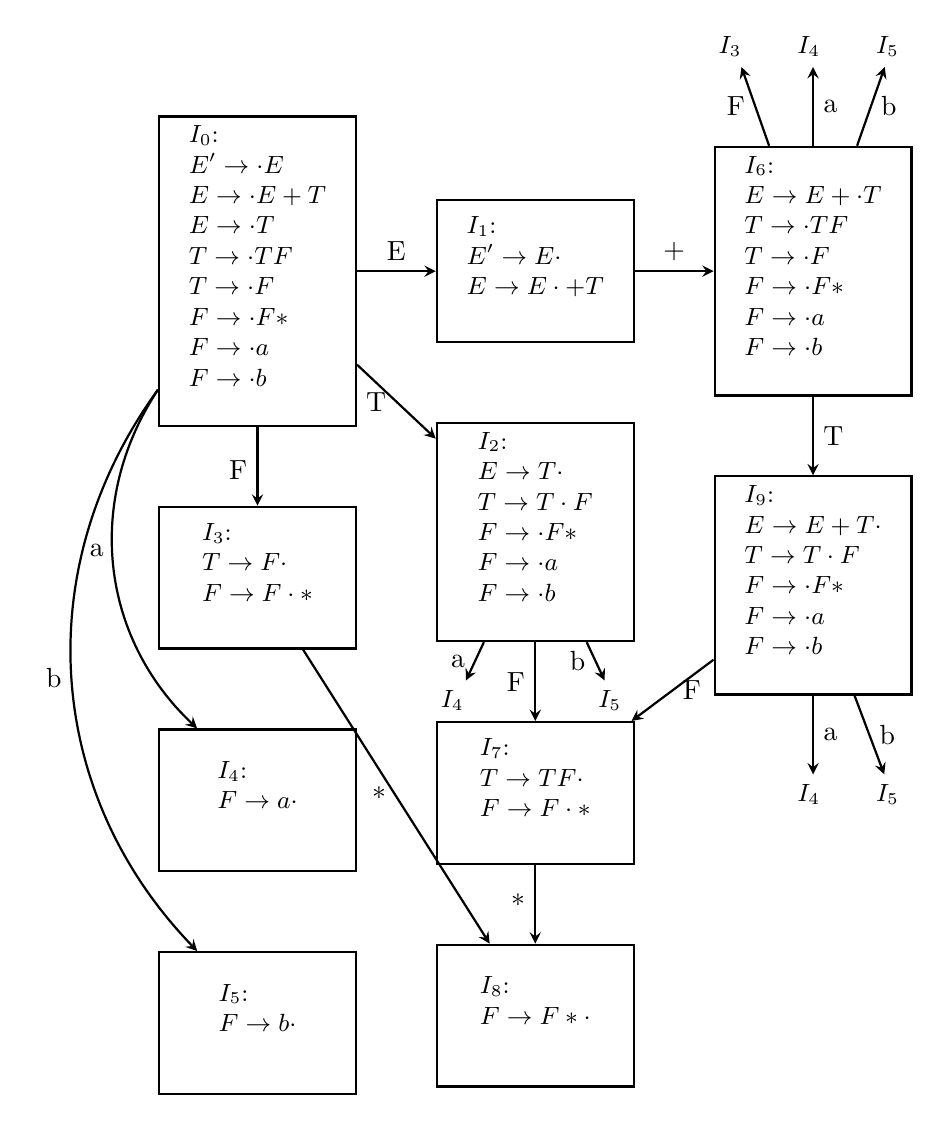
\begin{tikzpicture}[node distance=1cm]

% State I0
\node[state] (I0) {
    $I_0$:\\
    $E' \rightarrow \cdot E$\\
    $E \rightarrow \cdot E + T$\\
    $E \rightarrow \cdot T$\\
    $T \rightarrow \cdot TF$\\
    $T \rightarrow \cdot F$\\
    $F \rightarrow \cdot F*$\\
    $F \rightarrow \cdot a$\\
    $F \rightarrow \cdot b$\\
};

% State I1
\node[state, right=of I0] (I1) {
    $I_1$:\\
    $E' \rightarrow E \cdot$\\
    $E \rightarrow E \cdot + T$\\
};

% State I2
\node[state, below=of I1] (I2) {
    $I_2$:\\
    $E \rightarrow T \cdot$\\
    $T \rightarrow T \cdot F$\\
    $F \rightarrow \cdot F*$\\
    $F \rightarrow \cdot a$\\
    $F \rightarrow \cdot b$\\
};

% State I6
\node[state, right=of I1] (I6) {
    $I_6$:\\
    $E \rightarrow E + \cdot T$\\
    $T \rightarrow \cdot TF$\\
    $T \rightarrow \cdot F$\\
    $F \rightarrow \cdot F *$\\
    $F \rightarrow \cdot a$\\
    $F \rightarrow \cdot b$\\
};

% State I9
\node[state, below=of I6] (I9) {
    $I_9$:\\
    $E \rightarrow E+T \cdot$\\
    $T \rightarrow T \cdot F$\\
    $F \rightarrow \cdot F*$\\
    $F \rightarrow \cdot a$\\
    $F \rightarrow \cdot b$\\
};

% State I3
\node[state, below=of I0] (I3) {
    $I_3$:\\
    $T \rightarrow F \cdot$\\
    $F \rightarrow F \cdot *$\\
};

% State I7
\node[state, below=of I2] (I7) {
    $I_7$:\\
    $T \rightarrow TF \cdot$\\
    $F \rightarrow F \cdot *$\\
};

% State I8
\node[state, below=of I7] (I8) {
    $I_8$:\\
    $F \rightarrow F* \cdot$\\
};

% State I4
\node[state, below=of I3] (I4) {
    $I_4$:\\
    $F \rightarrow a \cdot$\\
};

% State I5
\node[state, below=of I4] (I5) {
    $I_5$:\\
    $F \rightarrow b \cdot$\\
};

\node[sstate, above=of I6, xshift=-1cm] (I3') {
    $I_3$
};
\node[sstate, above=of I6] (I4') {
    $I_4$
};
\node[sstate, above=of I6, xshift=1cm] (I5') {
    $I_5$
};

\node[sstate, above=of I7, yshift=-1cm, xshift=-1cm] (I4'') {
    $I_4$
};
\node[sstate, above=of I7, xshift=1cm, yshift=-1cm] (I5'') {
    $I_5$
};

\node[sstate, below=of I9] (I4''') {
    $I_4$
};
\node[sstate, below=of I9, xshift=1cm] (I5''') {
    $I_5$
};

% Arrows with labels
\draw[arrow] (I0) -- node[above] {E} (I1);
\draw[arrow] (I0) -- node[left] {T} (I2);
\draw[arrow] (I0) -- node[below left, pos=0.3] {F} (I3);
\draw[arrow] (I0) to[bend right=40] node[above left] {a} (I4);
\draw[arrow] (I0) to[bend right=40] node[left] {b} (I5);

\draw[arrow] (I1) -- node[above] {+} (I6);

\draw[arrow] (I2) -- node[left] {F} (I7);
\draw[arrow] (I2) -- node[left] {a} (I4'');
\draw[arrow] (I2) -- node[left] {b} (I5'');

\draw[arrow] (I6) -- node[right] {T} (I9);
\draw[arrow] (I6) -- node[left] {F} (I3');
\draw[arrow] (I6) -- node[right] {a} (I4');
\draw[arrow] (I6) -- node[right] {b} (I5');

\draw[arrow] (I9) -- node[right] {F} (I7);
\draw[arrow] (I9) -- node[right] {a} (I4''');
\draw[arrow] (I9) -- node[right] {b} (I5''');

\draw[arrow] (I3) -- node[left] {*} (I8);

\draw[arrow] (I7) -- node[left] {*} (I8);

\end{tikzpicture}

\newpage

SLR分析表:

\begin{center}
    \begin{tabular}{|c|ccccc|ccc|}
        \hline
        & \multicolumn{5}{c|}{ACTION} & \multicolumn{3}{c|}{GOTO} \\
        \hline
         & $+$ & $*$ & $a$ & $b$  & \$ & $E$ & $T$ & $F$ \\
        \hline
        0 & & & $s_4$ & $s_5$ & & 1 & 2 & 3 \\
        1 & $s_6$ & & & & $acc$ & & & \\
        2 & $r_2$ & & $s_4$ & $s_5$ & $r_2$ & & & 7 \\
        3 & $r_4$ & $s_8$ & $r_4$ & $r_4$ & $r_4$ & & & \\
        4 & $r_6$ & $r_6$ & $r_6$ & $r_6$ & $r_6$ & & & \\
        5 & $r_7$ & $r_7$ & $r_7$ & $r_7$ & $r_7$ & & & \\
        6 & & & $s_4$ & $s_5$ & &  & 9 & 3 \\
        7 & $r_3$ & $s_8$ & $r_3$ & $r_3$ & $r_3$ & & & \\
        8 & $r_5$ & $r_5$ & $r_5$ & $r_5$ & $r_5$ & & & \\
        9 & $r_1$ & & $s_4$ & $s_5$ & $r_1$ &  &  & 7 \\
        \hline
    \end{tabular}
\end{center}


\subsection*{2. 对下面文法, 证明他是LL(1)文法,但不是 SLR 文法。}

$$
\begin{aligned}
    & S \to AaAb \mid BbBa \\
    & A \to \varepsilon \\
    & B \to \varepsilon \\
\end{aligned}
$$

\noindent\textbf{{\heiti 解答}}

FIRST 集:

\[
\begin{aligned}
    & FIRST(S) = \{a, b\} \\
    & FIRST(A) = \{\varepsilon\} \\
    & FIRST(B) = \{\varepsilon\} \\
\end{aligned}
\]

FOLLOW 集:

\[
\begin{aligned}
    & FOLLOW(S) = \{\$ \} \\
    & FOLLOW(A) = \{a, b\} \\
    & FOLLOW(B) = \{a, b\} \\
\end{aligned}
\]

预测分析表:

\begin{center}
    \begin{tabular}{|c|ccc|}
        \hline
        & $a$ & $b$ & \$ \\
        \hline
        $S$ & $S \to AaAb$ & $S \to BbBa$ & \\
        $A$ & $A \to \varepsilon$ & $A \to \varepsilon$ & \\
        $B$ & $B \to \varepsilon$ & $B \to \varepsilon$ & \\
        \hline
    \end{tabular}
\end{center}

所以是 LL(1) 文法。

增广文法:

\rstprc

$$
\begin{aligned}
    & \prc S' \to S \\
    & \prc S \to AaAb\\
    & \prc S \to BbBa \\
    & \prc A \to \varepsilon \\
    & \prc B \to \varepsilon \\
\end{aligned}
$$


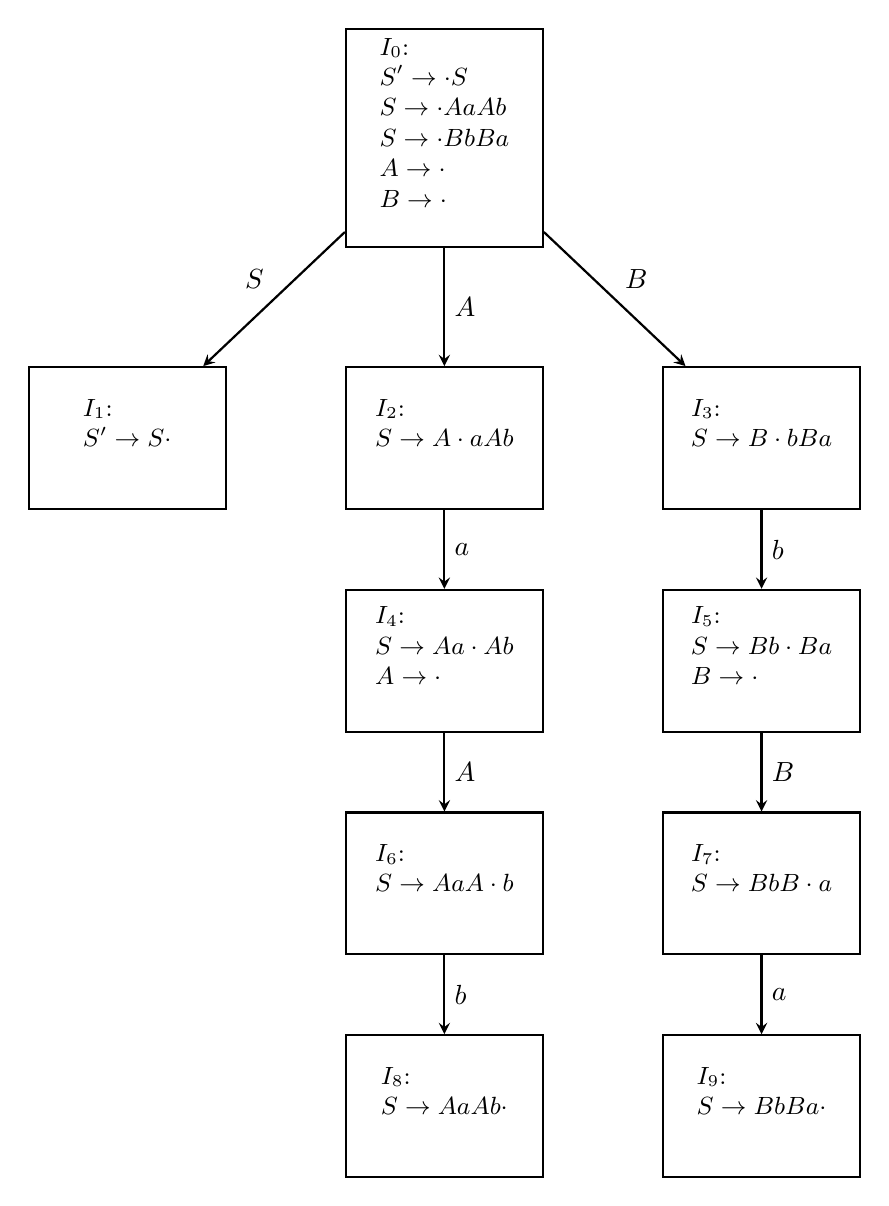
\begin{tikzpicture}[node distance=1cm]

% State I0
\node[state] (I0) {
    $I_0$:\\
    $S' \rightarrow \cdot S$\\
    $S \rightarrow \cdot AaAb$\\
    $S \rightarrow \cdot BbBa$\\
    $A \rightarrow \cdot$\\
    $B \rightarrow \cdot$\\
};

% State I1
\node[state, below left=1.5cm and 1.5cm of I0] (I1) {
    $I_1$:\\
    $S' \rightarrow S \cdot$\\
};

% State I2
\node[state, right=1.5cm of I1] (I2) {
    $I_2$:\\
    $S \rightarrow A \cdot aAb$\\
};

% State I3
\node[state, right=1.5cm of I2] (I3) {
    $I_3$:\\
    $S \rightarrow B \cdot bBa$\\
};

% State I4
\node[state, below=of I2] (I4) {
    $I_4$:\\
    $S \rightarrow Aa \cdot Ab$\\
    $A \rightarrow \cdot$\\
};

% State I5
\node[state, below=of I3] (I5) {
    $I_5$:\\
    $S \rightarrow Bb \cdot Ba$\\
    $B \rightarrow \cdot$\\
};

% State I6
\node[state, below=of I4] (I6) {
    $I_6$:\\
    $S \rightarrow AaA \cdot b$\\
};

% State I7
\node[state, below=of I5] (I7) {
    $I_7$:\\
    $S \rightarrow BbB \cdot a$\\
};

% State I8
\node[state, below=of I6] (I8) {
    $I_8$:\\
    $S \rightarrow AaAb \cdot$\\
};

% State I9
\node[state, below=of I7] (I9) {
    $I_9$:\\
    $S \rightarrow BbBa \cdot$\\
};

% Arrows with labels
\draw[arrow] (I0) -- node[above left] {$S$} (I1);
\draw[arrow] (I0) -- node[right] {$A$} (I2);
\draw[arrow] (I0) -- node[above right] {$B$} (I3);

\draw[arrow] (I2) -- node[right] {$a$} (I4);
\draw[arrow] (I3) -- node[right] {$b$} (I5);

\draw[arrow] (I4) -- node[right] {$A$} (I6);
\draw[arrow] (I5) -- node[right] {$B$} (I7);

\draw[arrow] (I6) -- node[right] {$b$} (I8);
\draw[arrow] (I7) -- node[right] {$a$} (I9);

\end{tikzpicture}

由于 $I_0$ 中存在 reduce/reduce 冲突,所以不是 SLR文法。

\end{document}
